\chapter{Manejo de bibliografía}



Sí, sí, a lo largo del documento hemos estado citando fuentes, esos números entre corchetes que evitan que nos demanden por plagio.

Aunque en este documento lo explicamos después de todas las desventuras relacionadas al contenido, espero que tengas un compendio de todas las fuentes que has utilizado para tu tesis, para solo venir a vaciar la información en un formato que \LaTeX{} entienda.

Lo bueno es que todo se reduce a crear un archivo de fuentes (o varios) y compilar... más o menos como lo hemos venido haciendo. Dependiendo de tu compilador, los pasos no cambian, al menos superficialmente.

Por supuesto, no todo es tan fácil como agregar un archivo con las fuentes con un |\input|, ni puedes utilizar las instrucciones |\label| en conjunto con |\ref|... así no funciona la cosa.

Antes de frustrarte con la explicación de cómo se hace, me gustaría contarte el motivo por el cual las referencias no se insertan así de simple (esperando que así no odies tanto a \LaTeX{} por su complejidad aparente).

Y sí, antes de empezar formalmente el capítulo quiero aclararlo: sí, la mayoría de las fuentes son digitales. Sí, rara vez se cita ya un libro. Sí, ``fuentes bibliográficas'' parece un término anacrónico e incorrecto, así como ``bibliografía''. Aún así, es lo que hay. Bienvenido al manejo de la bibliografía, aunque en tus fuentes no existan libros siquiera.



\section{¿Por qué las fuentes precisan otras instrucciones?}
\label{sec:_por_que_las_referencias_precisan_de_diferentes_instrucciones}



Si es tu primer trabajo en \LaTeX{}, y además tu primera investigación formal, entonces no tienes mucha idea de lo que son las fuentes y por qué son importantes (aunque, sí, básicamente se reduce a evitar demandas por plagio...).

En sí, las investigaciones formales tienen su conjunto de reglas en cuanto al contenido y al formato, cosa que hemos cubierto a lo largo de este libro. Eso es obvio, ¿cómo hacer un documento sin un estándar a seguir?

Lo que resulta menos obvio es que también para citar o hacer referencia a otros trabajos se requiere de todo un estándar. Sí, todo un \st{maldito}\footnote{Perdón, tengo sentimientos muy fuertes al respecto.}\textsuperscript{,}\footnote{Mi editor dijo que esta palabra no entraba en una publicación de tintes académicos, así que no está aquí.} estándar para mostrar las referencias a otras publicaciones, libros, páginas de Internet, publicación periódica... en fin, todo un arte.

Y sí, no estoy exagerando con que se podría escribir todo un libro nada más para citar correctamente. Si no me crees, puedes buscar sobre el formato APA\footnote{Del inglés \emph{American Psychological Association}} para referencias, definidas en un libro llamado ``Publication Manual of the American Psychological Association'' \cite{bib:apa}. Por supuesto, no es un libro sobre cómo citar exclusivamente, pero es un ejemplo de lo mucho que te puedes perder en un tema que parece tan insignificante.

Como este es un libro orientado a tesis de ingeniería, estoy casi seguro que a lo largo de la carrera viste artículos de la IEEE o Elsevier. O incluso libros de editoriales como Springer, donde había referencias salpicadas a lo largo del texto, con numeritos entre corchetes. Algo así como el siguiente texto:

\begin{displayquote}
En trabajos como [3] y [4] se tomó la aproximación por vida media. No obstante, trabajos como [5] y [6] demuestran que bajo condiciones de baja luminosidad, los resultados divergen.
\end{displayquote}

Claro, ese enunciado carece de sentido, pero así se leen la mayoría de los artículos académicos que igual no comprendemos (pero deberíamos de).

Y, bueno, ¿eso qué tiene que ver con \LaTeX{} o la forma en la que se citan las fuentes? En ingeniería es muy común hacer referencias con numeritos, como en el ejemplo anterior, porque somos más pragmáticos.

Por otro lado, si fuesemos a mostrar el mismo ejemplo anterior con el formato APA, luciría algo así:

\begin{displayquote}
En trabajos como (Mitchell, 2018) y (Stevensons, 2019) se tomó la aproximación por vida media. No obstante, trabajos como (Cloude y Papathanassiou, 2018) y (Rosen et al., 2000) demuestran que bajo condiciones de baja luminosidad, los resultados divergen.
\end{displayquote}

Como puedes ver, esos de la Asociación Estadounidense de Psicología son menos prácticos que nosotros los ingenieros (diría que más ególatras porque quieren ver sus nombres en cada cita pero... no, solo menos prácticos).

Como \LaTeX{} no fue concebido para uso exclusivo de ingeniería, e incluso nosotros nos tenemos que manchar las manos con ese ridículo formato de referencias mal concebido por la APA, ¿cómo le hacemos para saber si usamos APA o IEEE? ¿Cómo cambiamos fácilmente de un estilo a otro?

Es hora de un nuevo personaje en este ya-no-tan breve cuento de \TeX...



\section{\BibTeX}
\label{sec:bibtex}



En el capítulo \ref{cha:introduccion} aprendimos que existían \TeX{} y \LaTeX{}, así como otras cosas arcanas en las que no nos íbamos a meter... sí... este... mentí. Llegó la hora de agregar otro \TeX{} a nuestro cinturón de cosas por aprender, porque para las referencias tenemos algo llamado \BibTeX.

¿Qué es y por qué existe \BibTeX? Como vimos en el apartado anterior, la presentación de las referencias varía según el formato que se nos pida. La información que tienen es la misma, en el sentido que el libro o artículo sigue teniendo el mismo título, pero no la misma forma de presentarse (llámese formato IEEE o APA).

En síntesis, \BibTeX{} es la respuesta a la pregunta de ``¿cómo hacer un compendio de referencias que tenga la misma información pero varíe la forma de presentarlas?''. Es decir, podemos capturar la referencia a la página de \BibTeX{} con el siguiente código:

\begin{lstlisting}[style=bibtex]
@misc{bib:bibtex,
  title = {Your BibTeX resource},
  howpublished = {\url{http://www.bibtex.org/}},
  note = {Accedido: 2020-11-26}
}
\end{lstlisting}

\noindent y realmente no importa cómo lo tengamos que desplegar, podemos utilizar el comando |\cite{bib:bibtex}| para que aparezca la referencia en el formato que especifiquemos. En este libro, configurado en formato IEEE, ese comando me imprime estos corchetes \cite{bib:bibtex}.

La definición más formal, de acuerdo al sitio oficial, es la siguiente:

\begin{displayquote}
\BibTeX{} es tanto una herramienta como un formato de archivo usados para describir y procesar una lista de fuentes, la mayoría de las veces en conjunto con \LaTeX{}.
\end{displayquote}

Ese parrafito nos quiere decir tres cosas. Primero, que la parte de ``herramienta'' hace referencia a un compilador especial. Sí, al compilar \LaTeX{} en realidad estás ejecutando más procesos, pero son abstraídos de la mayoría de las interfaces gráficas.

Durante todo este tiempo hemos estado corriendo la herramienta \texttt{pdflatex}, que compila \LaTeX{} a un documento PDF (de ahí el nombre). Pero resulta que para agregar fuentes es necesario llamar al compilador de fuentes, llamado \texttt{bibtex}, y posteriormente reconstruir el PDF mandando llamar otra vez a \texttt{pdflatex}.

Espera, ¿qué? Sí, así como lo lees. Compilas el documento, luego las fuentes, luego vuelves a compilar el documento. Como usuario final, este proceso ocurre transparente para ti, pero está sucediendo cada vez que compilas.

Pero, ¿por qué sería necesario este absurdo juego de compilar el PDF una vez, luego compilar las fuentes, y luego el PDF otra vez?

Parte de la explicación está en saber que \BibTeX{} no te va a reportar una fuente que no mandaste llamar. Es decir, si tienes un archivo con 50 fuentes bibliográficas, pero en tu documento mandas llamar 30, entonces te regresará esas treinta que efectivamente utilizaste.

¿Para qué imprimir todas las cincuenta referencias si ni tú sabes el contexto o el por qué las incluiste? Las personas que lean tu documento no sabrán por qué o cómo es que hay veinte fuentes sin utilizar, ni les interesará. Es más, si no están asociadas al texto, ni las verán. O, dime, ¿cuándo fue la última vez que te pusiste a revisar la bibliografía, especialmente para buscar fuentes sin referencia en el artículo o libro? Exacto.

Entonces, la primer compilación con \texttt{pdflatex} es un barrido para hacer una lista con todas las fuentes que referencias, para luego mandar esa lista a \BibTeX. Luego, el compilador \texttt{bibtex} realiza una búsqueda en su almacen para ver si tiene lo que le pides. Si sí, regresa la información. Caso contrario, imprime una advertencia de que la fuente no fue encontrada.

Posteriormente, la nueva compilación con \texttt{pdflatex} colocará las referencias con la información que regresó \texttt{bibtex}, ya sea un número entre corchetes, nombres de los autores entre paréntesis, o algún otro formato de los disponibles.

El segundo dato que la definición formal arroja es que \BibTeX{} es una herramienta independiente de \LaTeX{}, y se puede emplear con otro tipo de documentos. Como ya vimos, el compilador \texttt{bibtex} funge como buscador de las fuentes que le piden, y esa funcionalidad se puede usar de manera independiente.

De cualquier forma, en este libro solo nos planteamos su uso con \LaTeX{}, así que lo demás no importa. Por último, tenemos que \BibTeX{} también es un tipo de archivo, que es lo que cubriremos a continuación.


\section{Archivo de bibliografía}
\label{sec:archivo_de_bibliografia}



Para empezar, un archivo de bibliografía tiene la extensión \texttt{.bib}. Como en este libro no nos complicamos la existencia, el archivo de bibliografía se llama \texttt{bibliografía.bib}.

Este archivo contiene texto plano, como los archivos \texttt{.tex}, y lo puedes editar hasta en bloc de notas. Si esperabas un asistente para dar de alta tus fuentes, de nuevo estás sin suerte.

Para incluir este archivo a nuestro documento se requieren dos instrucciones, ninguna de las cuales es |\input|. La primer instrucción tiene que ver con incluir el archivo tal cual, lo que hacemos con la instrucción |\bibliography| y el nombre del archivo entre llaves, sin la extensión. Algo así:

\begin{lstlisting}[style=latex]
\bibliography{bibliografia}
\end{lstlisting}

No obstante, hasta este punto \LaTeX{} no sabe cómo se van a mostrar esas fuentes en el texto. ¿Como IEEE, como APA, como algo más? Hasta no saber, \LaTeX{} no hará nada. Y no, no tiene un valor predeterminado para esto. Si no le especificas cómo representar la información que \BibTeX{} regresa, tu documento no tendrá referencias, y lo único que verás en la bitácora de compilación serán muchas advertencias, una por cada fuente bibliográfica que no fue encontrada:

\begin{lstlisting}[style=advertencias,mathescape=true]
LaTeX Warning: Citation `bib:opciones_spanish' on page 14 undefined.
LaTeX Warning: Citation `bib:emph' on page 15 undefined.
LaTeX Warning: Citation `bib:overleaf_emph' on page 15 undefined.
LaTeX Warning: Citation `bib:quotes' on page 16 undefined.
LaTeX Warning: Citation `bib:overleaf_lists' on page 23 undefined.
\end{lstlisting}

Esto en realidad no es un problema, simplemente debes especificar en qué formato quieres que se citen las fuentes. Los posibles valores son: \texttt{abbrv}, \texttt{acm}, \texttt{alpha}, \texttt{apalike}, \texttt{ieeetr}, \texttt{plain}, \texttt{siam}, y \texttt{unsrt}. Puedes ver cómo se ve cada una en \cite{bib:overleaf_bibtex}. El estilo seleccionado en este documento es \texttt{ieeetr}, lo cual en código luce así:

\begin{lstlisting}[style=latex]
% \bibliographystyle{estilo_a_usar}
\bibliographystyle{ieeetr}
\end{lstlisting}

Generalmente, la bibliografía es lo último que se imprime en una tesis (o libro), así que estas dos instrucciones suelen venir justo antes del |\end{document}|:

\begin{lstlisting}[style=latex]
\bibliographystyle{ieeetr}
\bibliography{bibliografia}

\end{document}
\end{lstlisting}



\section{Tipos de fuentes bibliográficas}
\label{sec:tipos_de_fuentes_bibliograficas}



Es hora de llenar el compendio de fuentes bibliográficas. Lo primero que hay que saber es qué tipo de fuentes acepta. ¿Puedo agregar libros, películas, artículos, páginas web? ¿Qué está permitido y qué no?

Aquí es donde volvemos a notar el anacronismo: la mayoría de fuentes bibliográficas soportadas directamente son documentos de papel, o documentos surgidos de algún evento de carácter científico.

¿A qué me refiero? Hay catorce tipos de fuente, detalladas en \cite{bib:overleaf_bibtex}, de las cuales tres tienen que ver con congresos (\texttt{conference}, \texttt{inproceeding}, y \texttt{proceedings}), dos tienen que ver con tesis (\texttt{masterthesis} y \texttt{phdthesis}) y otras dos tienen que ver con documentos técnicos (\texttt{manual} y \texttt{techreport}).

Eso nos deja con siete tipos, aunque realmente otros tres se parecen mucho: \texttt{book}, \texttt{inbook}, e \texttt{incollection}. Estos hacen referencia a un libro, a una sección de un libro (como un capítulo), y a una parte del libro (como una historia dentro de la colección).

Quedan cuatro: artículo (\texttt{article}), libreto (\texttt{booklet}, como un libro de menos prestigio), miscelánea (\texttt{misc}), y documento no publicado (\texttt{unpublished}, o manuscritos).

Para tu tesis, la mayoría de referencias debería venir de artículos y conferencias, preferentemente. Tal vez requieras referenciar algunas tesis de tu institución porque continúas el trabajo de años en una línea particular de investigación. En menor medida, tu apoyo vendrá de libros.

¿Pero qué pasa si tienes que citar un video o una página web? En ese caso, tu opción será el tipo \texttt{misc}. Aunque las fuentes en línea siguen teniendo cierto estigma, ya existe mucha más información y presencia en línea, ya sea de fabricantes de equipo especializado, editoriales, o autores de libros. Debido a esto, ya no es tanto problema utilizar este tipo de referencias\footnote{Pero, por favor, que el 90\% de tu bibliografía no sea Wikipedia.}. No obstante, un trabajo con mejores credenciales, que haya pasado por un mayor escrutinio, siempre será preferido sobre uno con menos referencias (en dos sentidos: tener fuentes que lo respalden y a su vez ser citado por otros).

Habiendo dicho esto, veamos cómo dar de alta nuestras fuentes bibliográficas.



\subsection{El formato general de una fuente}
\label{sub:el_formato_general_de_una_fuente}


Para dar de alta una entrada en la bibliografía primero necesitamos saber su tipo. Aquí lidiaremos solo con cinco: \texttt{article}, \texttt{inproceedings}, \texttt{book}, \texttt{masterthesis} y \texttt{misc}. Lo segundo que necesitamos saber es qué nombre o identificador le pondremos. Es decir, lo que usaremos para que \LaTeX{} genere la referencia a nuestra fuente. Entonces, el esqueleto luce así:

\begin{lstlisting}[style=bibtex]
@tipo_de_fuente{bib:identificador,
	% Atributos propios de la fuente.
}
\end{lstlisting}

No es necesario que el identificador inicie con \texttt{bib:} pero es un consenso extraoficial de la comunidad de \LaTeX{}/\BibTeX{}. Dentro de esas llaves van los atributos, mismos que dependen del tipo de fuente que se use.

Antes de entrar en materia de los atributos, podemos agregar una cita con el comando |\cite| y el identificador de la referencia:

\begin{lstlisting}[style=latex]
\cite{bib:identificador}
\end{lstlisting}

Como en este documento se maneja el estilo de la IEEE, el comando imprimirá el número asignado dentro de la bibliografía entre corchetes, como [núm]. Además, si se tiene cargado el paquete \texttt{hyperref}, ese numerito te llevará directo a la bibliografía, para que veas todos los datos de la fuente bibliográfica.

Ahora sí, veamos los atributos de los tipos de fuente que utilizaremos más.



\subsection{Atributos del tipo \texttt{article}}



El tipo \texttt{article} cuenta con cinco atributos requeridos: autor (\texttt{author}), título (\texttt{title}), publicación (\texttt{journal}), año (\texttt{year}), y volumen (\texttt{volume}). Opcionalmente puede contar número (\texttt{number}), y páginas (\texttt{pages}), entre otros, mismos que se pueden ver en la página de presentación del artículo en sitios como IEEE Xplore, como se muestra en la figura \ref{fig:ieee_ejemplo}.

\begin{figure}[ht!]
	\centering
	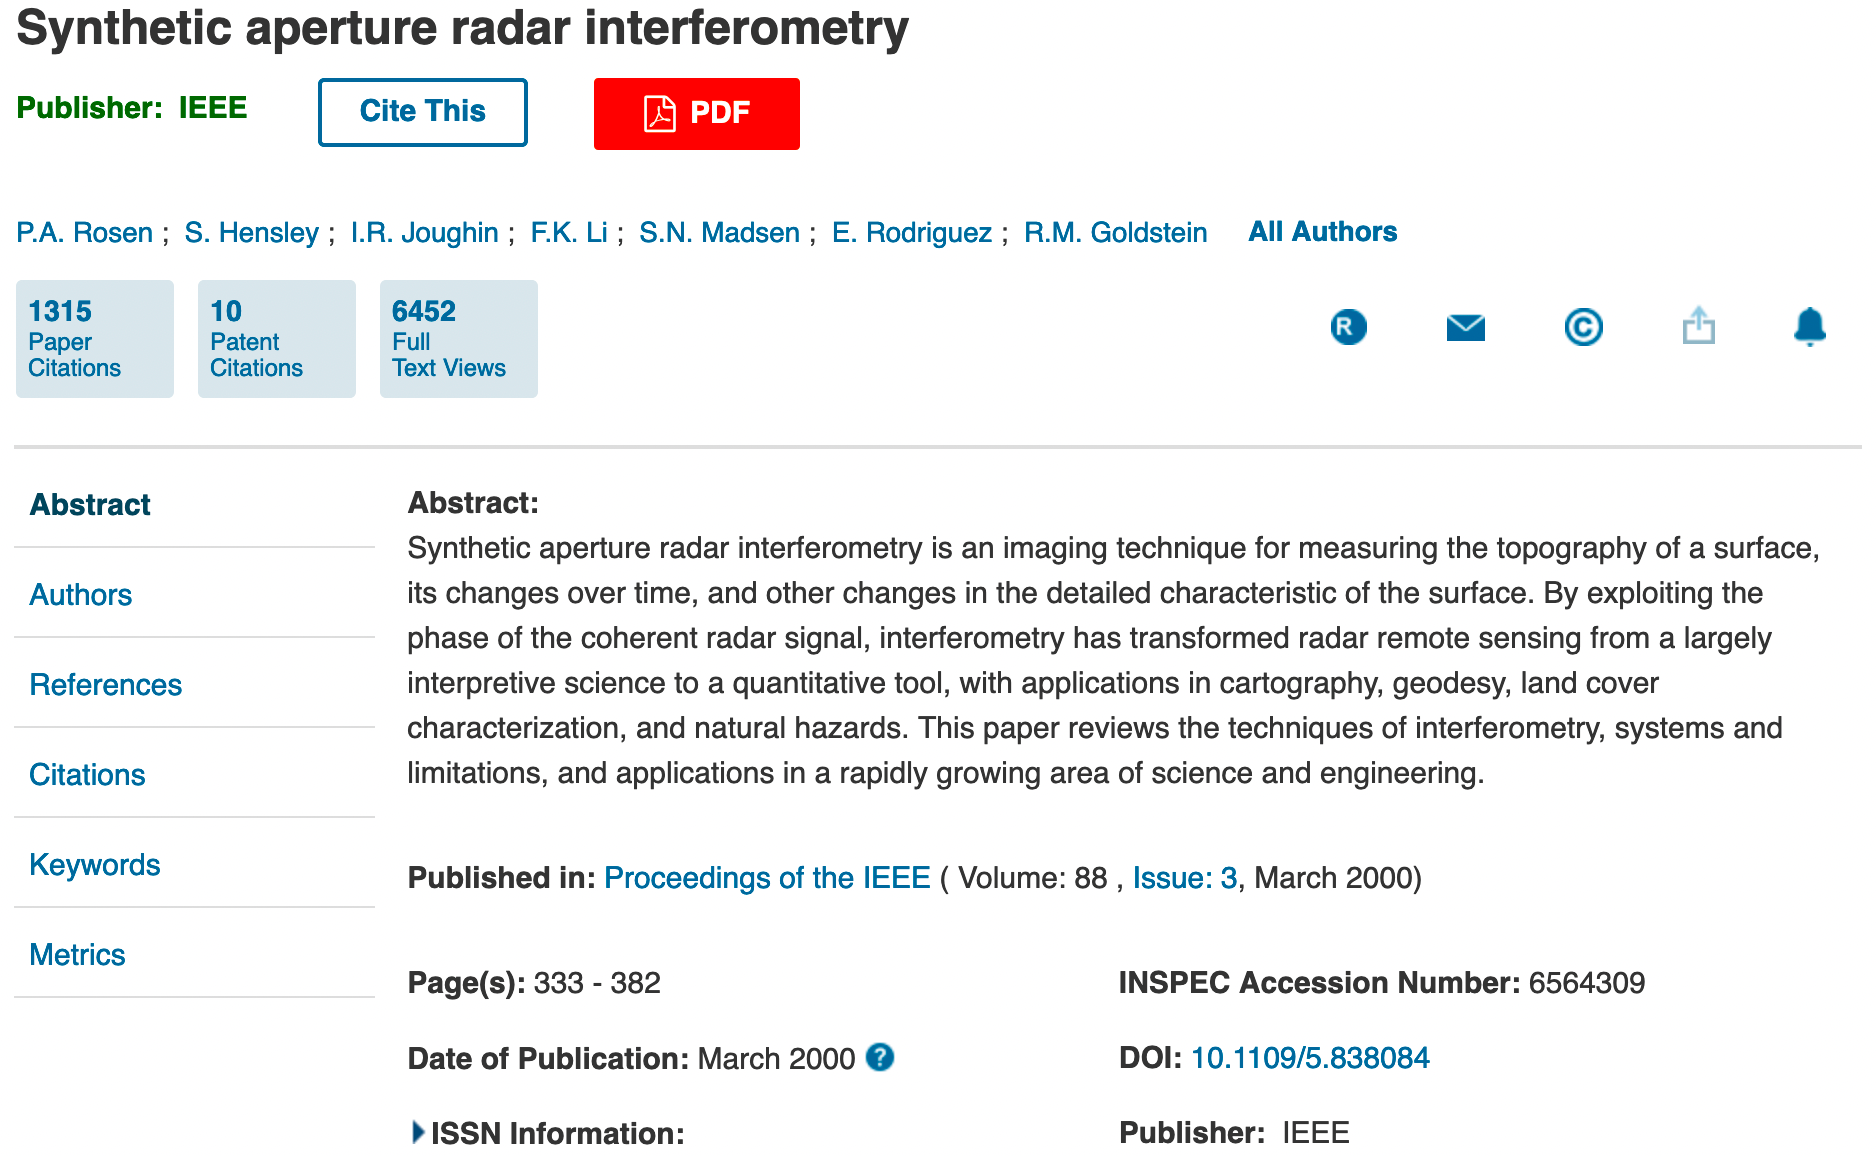
\includegraphics[width=\linewidth]{img/ejemplo_ieee_edit.png}
	\caption{Página de un artículo de la IEEE.}
	\label{fig:ieee_ejemplo}
\end{figure}

Pero IEEE Xplore no solo muestra la información en su página, también cuenta con el botón \opcionMenu{Cite this} para exportar la cita a \BibTeX{}. La figura \ref{fig:ieee_xplore_cite} muestra los atributos del artículo, listos para ser copiados y pegados, y el resultado se muestra en el listado \ref{lst:bibtex_ieee}.

\begin{figure}[ht!]
	\centering
	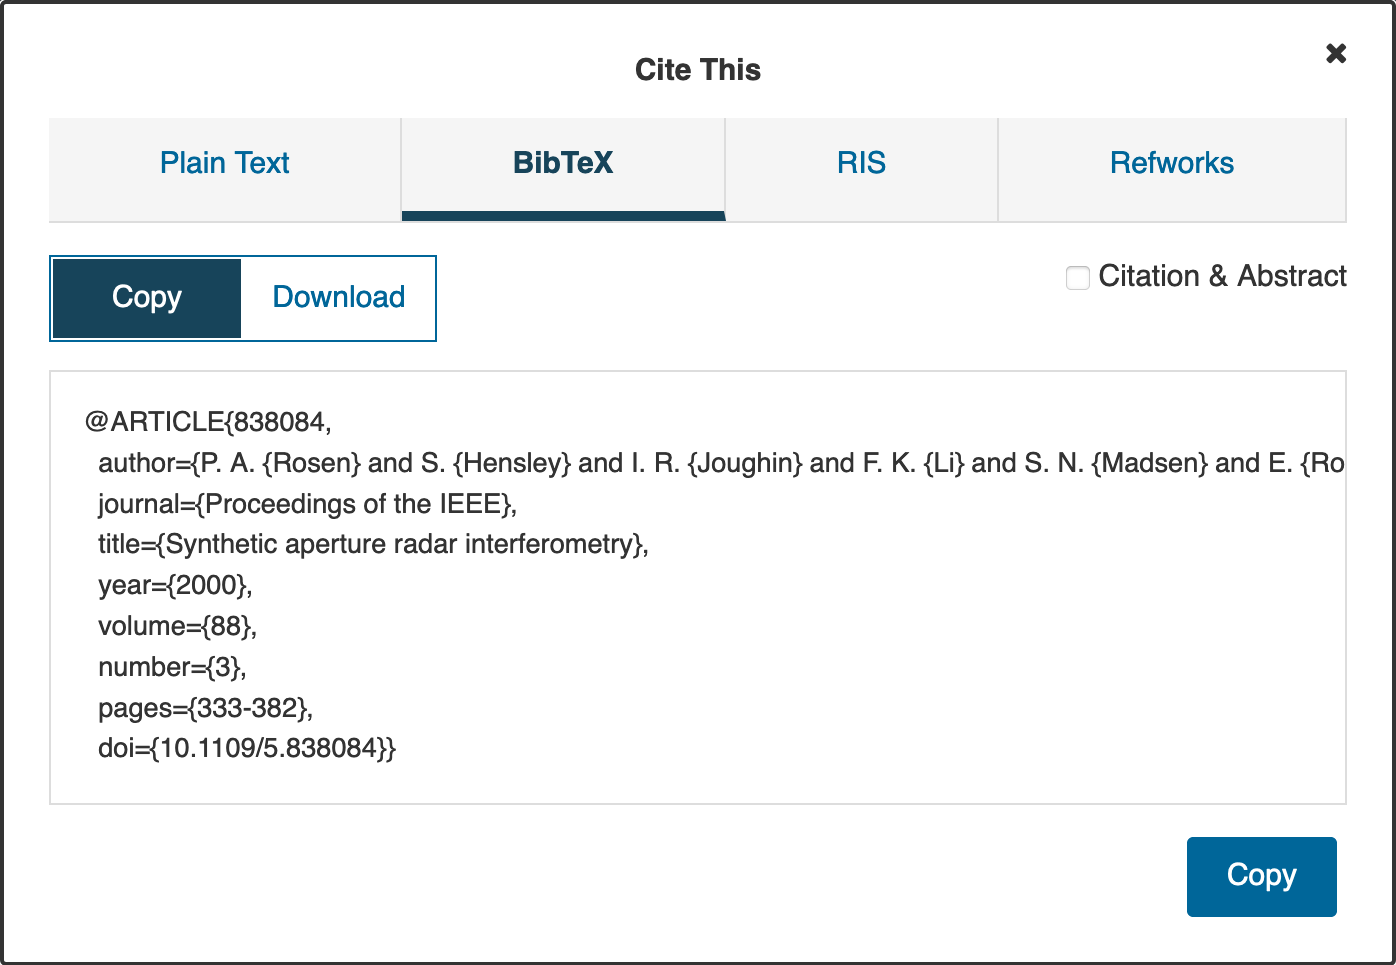
\includegraphics[width=0.70\linewidth]{img/ieee_xplore_cite.png}
	\caption{IEEE Xplore y su facilidad para exportar citas a \BibTeX{}.}
	\label{fig:ieee_xplore_cite}
\end{figure}

Lo primero que hay que mencionar del listado \ref{lst:bibtex_ieee} es que utiliza \texttt{@ARTICLE}, en mayúsculas. Esto es perfectamente válido, a \BibTeX{} no le importa si está en mayúsculas o minúsculas el tipo de fuente. En esa misma línea se encuentra el identificador asignado por la IEEE, el número \texttt{838084} (lo cual probablemente significa algo para ellos, pero no para nosotros). Puedes cambiar este identificador, sin problemas, por algo más fácil de recordar a la hora de citar, como \texttt{bib:radar}.

Lo segundo que hay que mencionar es que, de manera similar a los listados, los atributos de la fuente están separados por comas. Eso explica por qué todos los valores de los atributos están delimitados por un par de llaves, su función es proteger el valor del atributo en caso de que contenga comas (como el título del libro ``Comer, rezar, amar'').

Lo que llama más la atención es el atributo del autor por su gran cantidad de llaves. Esa explicación la guardaremos para la próxima sección. De momento podemos mencionar que la palabra \texttt{and} es una palabra clave reservada de \BibTeX{} que sirve para separar a los autores del artículo.

Finalmente, la entrada provista por la IEEE nos da el atributo \texttt{doi}, que proviene del inglés \emph{Digital Object Identifier}, mismo que identifica permanentemente un recurso en línea (el DOI no cambia, los URLs sí).

\begin{lstlisting}[style=bibtex,caption={Entrada de un artículo de la IEEE.},label=lst:bibtex_ieee]
@ARTICLE{838084,
	author={P. A. {Rosen} and S. {Hensley} and I. R. {Joughin} and F. K. {Li} and S. N. {Madsen} and E. {Rodriguez} and R. M. {Goldstein}},
	journal={Proceedings of the IEEE},
	title={Synthetic aperture radar interferometry},
	year={2000},
	volume={88},
	number={3},
	pages={333-382},
	doi={10.1109/5.838084}
}
\end{lstlisting}



\subsection{Atributos del tipo \texttt{inproceedings}}



Este tipo de entrada es sobre una publicación presentada en una serie de conferencias. Generalmente, dichas conferencias terminan en un bonito libro (pero sigue siendo un \texttt{inproceedings}). Este tipo de entrada comparte varios atributos con el \texttt{article}: \texttt{author}, \texttt{title}, \texttt{year}, y \texttt{pages}, y agrega otros propios de las conferencias: ¿dónde fue? (\texttt{address}), nombre del libro resultante (\texttt{booktitle}), serie a la que pertenece el libro (\texttt{series}), y editor (\texttt{publisher}).

\begin{figure}[ht!]
	\centering
	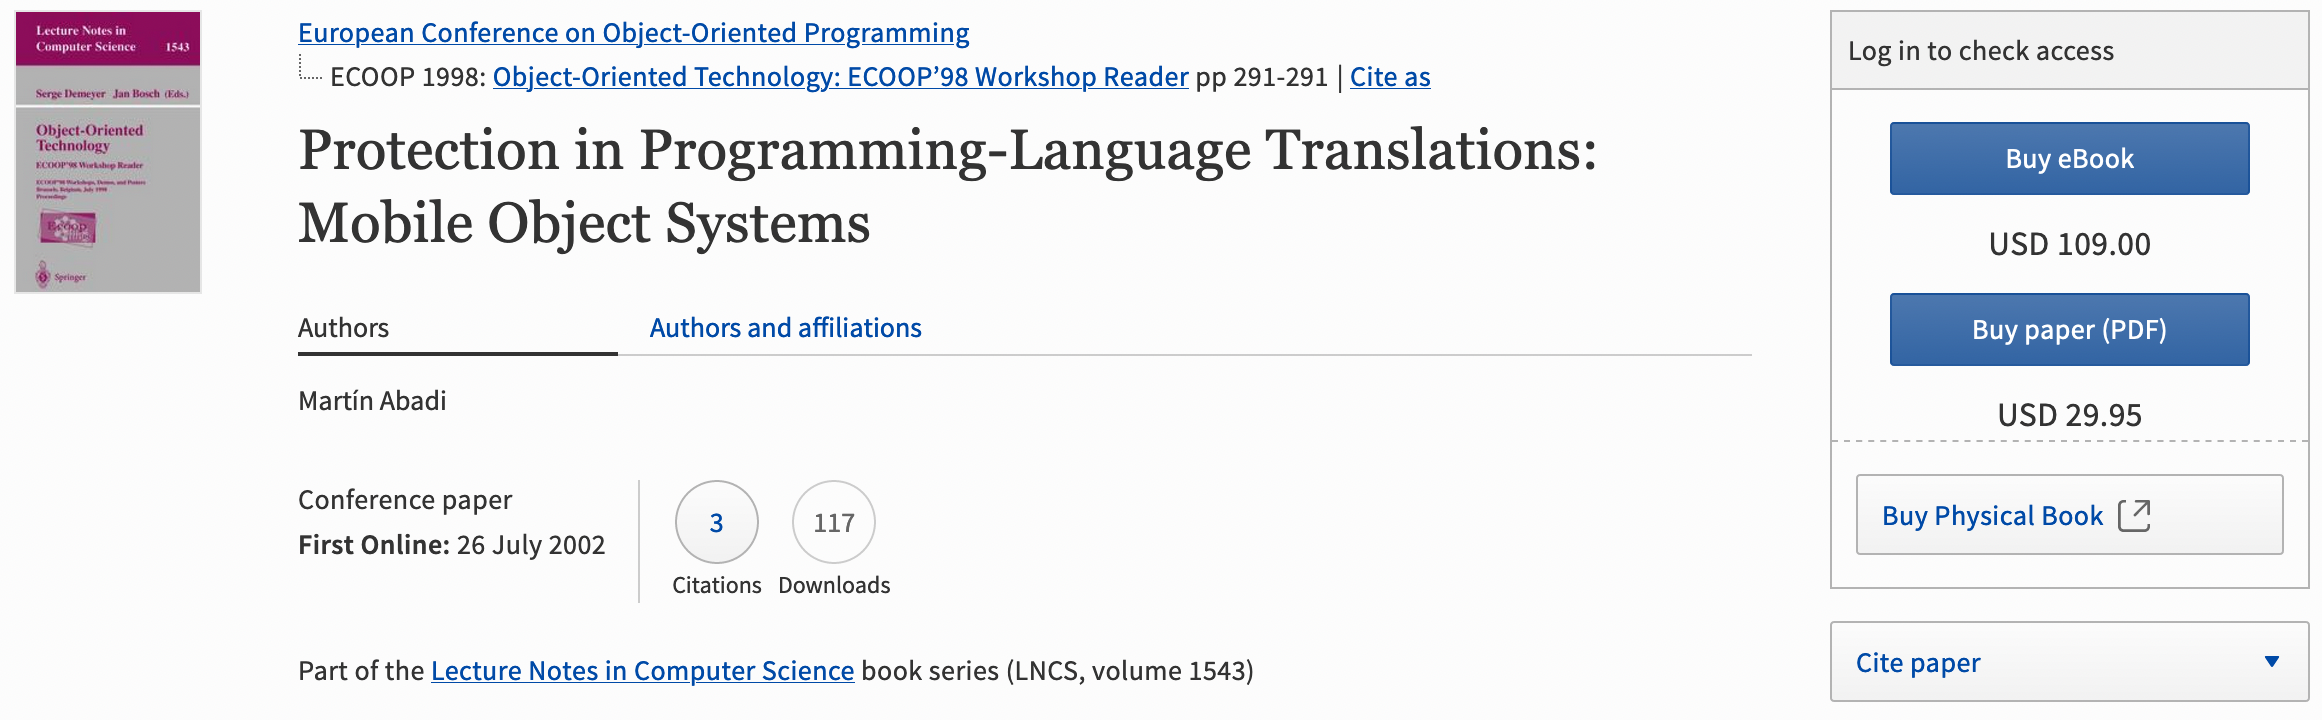
\includegraphics[width=\linewidth]{img/ejemplo_springer.png}
	\caption{Artículo de conferencia disponible en Springer.}
	\label{fig:ejemplo_springer}
\end{figure}

Un ejemplo de una entrada \texttt{inproceedings} se muestra en la figura \ref{fig:ejemplo_springer}, misma que muestra el botón de \opcionMenu{Cite paper} a la derecha, debajo de los botones de venta del libro completo. El código de la fuente bibliográfica provisto por Springer se muestra en el listado \ref{lst:bibtex_springer}. La primera línea muestra el tipo de fuente, en este caso \texttt{@InProceedings}. De nuevo, mayúsculas, minúsculas, o combinado, no importa para \BibTeX{}. Contrario al caso de la IEEE, Springer usa su DOI como identificador... aunque no lo pone como atributo de la fuente.

\begin{lstlisting}[style=bibtex,caption={Entrada de un artículo de Springer.},label=lst:bibtex_springer]
@InProceedings{10.1007/3-540-49255-0_70,
	author="Abadi, Mart{\'i}n",
	editor="Demeyer, Serge and Bosch, Jan",
	title="Protection in Programming-Language Translations: Mobile Object Systems",
	booktitle="Object-Oriented Technology: ECOOP'98 Workshop Reader",
	year="1998",
	publisher="Springer Berlin Heidelberg",
	address="Berlin, Heidelberg",
	pages="291--291",
	abstract="We discuss abstractions for protection and the correctness of their implementations. Relying on the concept of full abstraction, we consider several examples relevant to mobile object systems. The main example is the translation of Java classes to an intermediate bytecode language. Other examples are the implementation of procedures by closures and the implementation of private communication channels in terms of cryptographic operations.",
	isbn="978-3-540-49255-9"
}
\end{lstlisting}

Además, esta entrada contiene más atributos que los anteriormente mencionados, como son \texttt{editor}, \texttt{abstract}, e \texttt{isbn}. El hecho de que tenga más atributos no significa que serán impresos a la hora de imprimir la bibliografía, así que no hacen daño.

Otra cosa a considerar es que en esta entrada se usan comillas para delimitar los valores de los atributos, en lugar de llaves. Y sí, también es totalmente válido.

Finalmente... sí, esta entrada lista los editores con el formato \emph{Apellido, Nombre}, mientras que la de IEEE era \emph{Nombre Apellido}, ¿transformamos manualmente de una a otra? De momento solo estamos viendo los valores de cada atributo, pero no terminaremos el capítulo sin más observaciones al respecto.



\subsection{Atributos del tipo \texttt{book}}



Hay que decirlo: lo más lamentable de incluir libros es que no existen botones que brinden toda la información de la obra para solo colocar en \BibTeX{} (lo sé, ya te estabas acostumbrando a ello). Posiblemente, esta es la razón por la que se deben incluir más artículos y conferencias, para evitar buscar la información necesaria para citar la fuente.

Fuera de bromas, para estas alturas nos hemos quedado sin nuevos atributos requeridos, al menos respecto a los ya vistos en el tipo \texttt{article} e \texttt{inproceedings}, pues un \texttt{book} debe contar con: \texttt{author} o \texttt{editor}, \texttt{title}, \texttt{year}, y \texttt{publisher}.

Por ejemplo, para hacer referencia al presente libro crearíamos una entrada como se muestra en el listado \ref{lst:bibtex_rc_latex}, misma que en la bibliografía se muestra con el número \cite{bib:latex_ingenieria}).

\begin{lstlisting}[style=bibtex,caption={Entrada de \BibTeX{} de un libro.},label=lst:bibtex_rc_latex]
@book{bib:latex_ingenieria,
  author="{Carlos Alberto} {Ramos López}",
  title="LaTeX para tesis de ingeniería",
  year="2021",
  publisher="Leanpub"
}
\end{lstlisting}



\subsection{Atributos del tipo \texttt{masterthesis}}



Una tesis de maestría se referencía con cuatro atributos requeridos: \texttt{author}, \texttt{title}, \texttt{school}, y \texttt{year}. El único atributo nuevo es la escuela, y probablemente solo tengas que utilizar referencias a tu institución educativa o aquellas universidades con las que trabajaste en conjunto (si es que las hay).

El listado \ref{lst:bibtex_rc_tesis} muestra el código para referenciar mi tesis de maestría, con el mínimo de datos capturado. Y sí, ese es el nombre completo de mi trabajo (que tiene asignado el numerito \cite{bib:ejemplo_tesis}). Continuemos.

\begin{lstlisting}[style=bibtex,caption={Entrada de una tesis de maestría.},label=lst:bibtex_rc_tesis]
@masterthesis{bib:ejemplo_tesis,
  author="{Ramos López}, {Carlos Alberto}",
  title="Diseño e Implementación de un Sistema basado en Nios II para la Captura y Procesamiento de Interferogramas en la Caracterización de MEMS",
  year="2014",
  school="Universidad Autónoma de Ciudad Juárez"
}
\end{lstlisting}



\subsection{Atributos del tipo \texttt{misc}}



Para el final dejamos el tipo \texttt{misc}, la panacea para todo lo demás, especialmente contenido en línea. Para citar una página web hacen falta tres atributos: el título de la página (\texttt{title}), el URL (mediante \texttt{howpublished}), y la fecha de acceso (mediante una \texttt{note}).

El atributo \texttt{howpublished} es el que contiene el enlace a la página web, a través del comando |\url| del paquete \texttt{hyperref}. En el listado \ref{lst:ejemplos_misc} se muestran dos ejemplos de contenido en línea.

\begin{lstlisting}[style=bibtex,numbers=left,caption={Entrada de dos recursos en línea.},label=lst:ejemplos_misc]
@misc{bib:overleaf_mathtools,
  title = {{Mathtools - for beautiful math}},
  howpublished = {\url{https://es.overleaf.com/learn/latex/Articles/Mathtools_-_for_beautiful_math}},
  note = {Accedido: 2020-12-22}
}
@misc{bib:math_cancel,
  title = {{The cancel package}},
  author = {Donald Arseneau},
  howpublished = {\url{http://ctan.math.washington.edu/tex-archive/macros/latex/contrib/cancel/cancel.pdf}},
  note = {Accedido: 2020-12-22}
}
\end{lstlisting}

El primer ejemplo, líneas 1 a 5, utiliza únicamente los tres atributos ``requeridos'' (es un tipo \texttt{misc}, en realidad no tiene requisitos). El segundo ejemplo agrega al autor del recurso en línea.

Por último, puedes consultar la lista completa de atributos en \cite{bib:bibtex_fields}. Dicha lista incluye atributos no mencionados aquí, como el \texttt{email} para capturar el correo electrónico del autor, o la \texttt{edition} para especificar la edición de un libro.

Es tiempo de responder por qué las líneas 2 y 7 de listado \ref{lst:ejemplos_misc}, correspondientes a los títulos, están encerradas entre doble llave.



\section{¿Por qué tanta llave?}
\label{sec:por_que_tanta_llave}



En los ejemplos de fuentes bibliográficas de este capítulo nos encontramos con doble llave en dos atributos en particular: \texttt{author} y \texttt{title}. En ambos casos podemos reducir la explicación a un simple enunciado: ``Deja el texto escrito tal y como está''.

Una de las tareas de \BibTeX{} es garantizar que todo esté con el formato correcto, y algunas veces eso significa que se toma privilegios para una tarea... y no sale bien. Uno de tales privilegios tiene que ver con las mayúsculas y minúsculas.

Si en \BibTeX{} colocas el título ``La defenestración de Ermintrude Inch'', \BibTeX{} aplicará una regla de ``¿Qué? ¿Solo la primera letra de toda la oración va mayúscula? Claro que sí, deja convierto en minúsculas todo lo demás'', dejando el nombre propio como ``ermintrude inch'', lo cual es incorrecto.

¿Qué se hace entonces? Se pone un par de llaves adicionales sobre aquello que se pretende proteger, aquello que no queremos que \BibTeX{} modifique. Puede ser sobre el nombre propio, \emph{Ermintrude Inch}, o sobre todo el contenido del atributo \texttt{title}. Para no batallar, lo más fácil es lo segundo. Para resumir:

\begin{lstlisting}[style=bibtex]
% Esto está mal, 'Ermintrude Inch' se transforma en 'ermintrude inch'.
title={La defenestración de Ermintrude Inch}
% Similar al caso anterior, el texto se transforma en 'ermintrude inch'.
title="La defenestración de Ermintrude Inch"
% Mal en muchos niveles, problemas de comillas (delimitan, no protegen).
title={La defenestración de "Ermintrude Inch"}
% Perfecto, las comillas delimitan, las llaves protegen las mayúsculas.
title="{La defenestración de Ermintrude Inch}"
% Perfecto, llaves externas delimitan, llaves del nombre lo protegen.
title={La defenestración de {Ermintrude Inch}}
% Perfecto, protege todo. Una exageración, pero funciona.
title={{La defenestración de Ermintrude Inch}}
\end{lstlisting}

Eso explica también las llaves alrededor de los apellidos de los autores. En el artículo de la IEEE, se puede ver que los apellidos de los autores están resguardados entre llaves:

\begin{lstlisting}[style=bibtex]
author={P. A. {Rosen} and S. {Hensley} and I. R. {Joughin} and F. K. {Li} and S. N. {Madsen} and E. {Rodriguez} and R. M. {Goldstein}},
\end{lstlisting}

\noindent pero no hay ninguna razón aparente para ello. No obstante, si consideras que las fichas para \BibTeX{} son generadas por algún script, todo cobra sentido. En inglés, no hay problema. Las personas tienen un apellido, y los que tienen más aprendemos a esconderlo (después de todo, mi nombre en Estados Unidos se limita a ``Carlos A. Ramos'').

Pero, siendo la IEEE un mecanismo internacional, se necesita garantizar que los apellidos de los autores se mantengan intactos. Así que, ¿qué se hace? Se protegen con llaves para que el apellido se imprima íntegro.

Eso explica porque mi apellido, \emph{Ramos López}, está encerrado entre llaves, así como mi nombre. Pero, para esa explicación mejor vayamos a la próxima sección.



\section{¿Nombre Apellido o Apellido, Nombre?}
\label{sec:nombre_apellido}



Si Springer me da las referencias con \emph{Apellido, Nombre}, y la IEEE como \emph{Nombre Apellido}, ¿cómo debo capturar yo las que restan? ¿Debo convertir de un formato a otro?

¿Recuerdas la parte donde nos complicamos la vida con \BibTeX{} y |\cite|? Es tiempo de que se nos retribuya por tanta complejidad: \BibTeX{} se encarga de todo. ¿Cómo?

Dentro de los ejemplos previos, la referencia al libro tiene como autor:

\begin{lstlisting}[style=bibtex]
author="{Carlos Alberto} {Ramos López}",
\end{lstlisting}

\noindent mientras que para la tesis tiene al autor declarado como \emph{Apellido, Nombre}:

\begin{lstlisting}[style=bibtex]
author="{Ramos López}, {Carlos Alberto}",
\end{lstlisting}

No obstante, al ver las entradas en la bibliografía podemos ver lo siguiente:

\vspace{10pt}
\noindent\begin{minipage}{0.05\linewidth}
\cite{bib:latex_ingenieria}\\
\cite{bib:ejemplo_tesis}\\
~\\
~
\end{minipage}
\begin{minipage}{0.9415\linewidth}
 C. Ramos López, \emph{LaTeX para tesis de ingeniería}. Leanpub, 2021.\\
 C. Ramos López, ``Diseño e Implementación de un Sistema basado en Nios II para la Captura y Procesamiento de Interferogramas en la Caracterización de MEMS,'' 2014.
\end{minipage}
\vspace{1pt}

Esas dos entradas ponen en evidencia tres cosas:
\begin{itemize}
	\item El orden de \emph{Nombre Apellido} o \emph{Apellido, Nombre} a la hora de la captura es irrelevante. \BibTeX{} va a reportar el nombre según el formato que le pidas.
	\item El apellido, \emph{Ramos López}, se mantuvo íntegro gracias a las llaves (y a que sí importa en las referencias en formato IEEE).
	\item Por otra parte, el nombre no importa, ni aunque esté entre llaves. El segundo nombre incluso desaparece, y el primer nombre queda reducido solo a una inicial.
\end{itemize}



\section{Múltiples autores y nombres con comas o ``and''}



Volvamos al ejemplo de múltiples autores, entrada listada con el número \cite{bib:radar}:

\begin{lstlisting}[style=bibtex]
author={P. A. {Rosen} and S. {Hensley} and I. R. {Joughin} and F. K. {Li} and S. N. {Madsen} and E. {Rodriguez} and R. M. {Goldstein}},
\end{lstlisting}

¿Ves presente alguna coma para separar a los autores? No. ¿Ves presente algún ``y'' para decir que es el último autor? Tampoco. Aún así, esa entrada se manifiesta así:

\vspace{10pt}
\noindent\begin{minipage}{0.05\linewidth}
\cite{bib:radar}\\
~\\
\end{minipage}
\begin{minipage}{0.9415\linewidth}
 P. A. Rosen, S. {Hensley}, I. R. Joughin, F. K. Li, S. N. {Madsen}, E. Rodriguez and R. M. Goldstein, ``Synthetic aperture radar interferometry,''	\emph{Proceedings of the IEEE}, vol. 88, no. 3, pp. 333-382, 2000.
\end{minipage}
\vspace{1pt}

Es decir, automáticamente \BibTeX{} separa los autores con comas y agrega un \emph{and} entre los dos últimos autores (sí, sí, eso nos da el problema de la traducción). El punto: separa los múltiples autores siempre con \texttt{and}.

Claro que hay otro problema. El hecho de que la coma se utilice para separar el apellido del nombre, y el \texttt{and} se utilice para separar autores, representa un problema a la hora de citar un trabajo cuyo autor es una organización, como \emph{Barnes and Noble, Inc}.

En base a lo que sabemos, \BibTeX{} pensará que son dos autores, uno llamado \emph{Barnes}, a secas, y otro llamado \emph{Inc. Noble} (de nuevo, apreciaciones incorrectas). La manera de evitar este comportamiento es protegiendo el nombre entre llaves, por ejemplo:

\begin{lstlisting}[style=bibtex]
author={{Barnes and Noble, Inc}},
\end{lstlisting}

\noindent y de esta manera no habrá ruptura en varios autores, ni evaluación de la coma. Todo ese nombre es parte de un único autor.



\section{Traducción}



La traducción del ``and'' a un ``y'' no es tan trivial como un |\renewcommand|. Para esta tarea hay que editar el archivo de definición del estilo \texttt{ieeetr}.

Si deseas saber todo el procedimiento para poder hacer cambios tú mismo al estilo, puedes consultar \cite{bib:bibtex_espanol}. En caso contrario, solo debes saber que el archivo \texttt{ieeetr.bst} que se encuentra en el repositorio de este libro hizo un cambio de ese ``and'' por un ``y''. Recuerda borrar archivos temporales antes de volver a compilar todo el documento.



\section{Otras opciones para compilar bibliografía}



Resulta que \BibTeX{} puede tener ciertas limitaciones con el ordenamiento de las fuentes bibliográficas en caso de querer ordenar por apellidos, o por otro criterio que no sea por orden de aparición (como en el estilo \texttt{ieeetr}).

En caso de que encuentres que \BibTeX{} es muy limitado para tus requerimientos, o difícil de configurar, existen otras opciones, como \BibLaTeX{}. Puedes consultar la documentación de Overleaf para su uso en \cite{bib:overleaf_biblatex}.



\section*{Resumen}



En este capítulo aprendimos cómo crear nuestra bibliografía por medio de \BibTeX{}, mismo que es una herramienta de compilación y un tipo de archivo a la vez.

Descubrimos que existen diversos estilos para citar fuentes, entre los cuales destacamos el de la IEEE y el formato APA, y que podemos elegir el estilo mediante la instrucción |\bibliographystyle{estilo_a_usar}|.

También aprendimos que el comando |\cite| nos permite referenciar una fuente declarada en nuestro compendio, y \LaTeX{} la imprimirá de acuerdo a los datos compilados mediante \BibTeX{}.

Además, aunque hay cierta complejidad al dar de alta las fuentes bibliográficas, desde determinar que tipo de fuente son hasta determinar sus atributos, existen páginas, como IEEE Xplore y Springer, que ya nos brindan toda la información con un par de clics.

Finalmente, lidiamos con unos cuantos problemitas propios de la lógica de \BibTeX{} a la hora de tratar con nombres, para así poder sacarle el máximo a sus facilidades sin sufrir mucho por sus aparentes defectos.

Lo único que resta es terminar unas cuantas secciones adicionales y enfocarnos un poco más en el formato.